%%%%%%%%%%%%%%%%%%%%%%%%%%%%%%%%%%%%%%%%%
% Beamer Presentation
% LaTeX Template
% Version 1.0 (10/11/12)
%
% This template has been downloaded from:
% http://www.LaTeXTemplates.com
%
% License:
% CC BY-NC-SA 3.0 (http://creativecommons.org/licenses/by-nc-sa/3.0/)
%
%%%%%%%%%%%%%%%%%%%%%%%%%%%%%%%%%%%%%%%%%

%----------------------------------------------------------------------------------------
%	PACKAGES AND THEMES
%----------------------------------------------------------------------------------------


%http://www.iep.utm.edu/mathplat/

\documentclass{beamer}

\mode<presentation> {

% The Beamer class comes with a number of default slide themes
% which change the colors and layouts of slides. Below this is a list
% of all the themes, uncomment each in turn to see what they look like.

%\usetheme{default}
%\usetheme{AnnArbor}
%\usetheme{Antibes}
%\usetheme{Bergen}
%\usetheme{Berkeley}
%\usetheme{Berlin}
%\usetheme{Boadilla}
%\usetheme{CambridgeUS}
%\usetheme{Copenhagen}
%\usetheme{Darmstadt}
%\usetheme{Dresden}
%\usetheme{Frankfurt}
%\usetheme{Goettingen}
%\usetheme{Hannover}
%\usetheme{Ilmenau}
%\usetheme{JuanLesPins}
%\usetheme{Luebeck}
\usetheme{Madrid}
%\usetheme{Malmoe}
%\usetheme{Marburg}
%\usetheme{Montpellier}
%\usetheme{PaloAlto}
%\usetheme{Pittsburgh}
%\usetheme{Rochester}
%\usetheme{Singapore}
%\usetheme{Szeged}
%\usetheme{Warsaw}

% As well as themes, the Beamer class has a number of color themes
% for any slide theme. Uncomment each of these in turn to see how it
% changes the colors of your current slide theme.

%\usecolortheme{albatross}
%\usecolortheme{beaver}
%\usecolortheme{beetle}
%\usecolortheme{crane}
%\usecolortheme{dolphin}
%\usecolortheme{dove}
%\usecolortheme{fly}
%\usecolortheme{lily}
%\usecolortheme{orchid}
%\usecolortheme{rose}
%\usecolortheme{seagull}
%\usecolortheme{seahorse}
%\usecolortheme{whale}
%\usecolortheme{wolverine}

%\setbeamertemplate{footline} % To remove the footer line in all slides uncomment this line
%\setbeamertemplate{footline}[page number] % To replace the footer line in all slides with a simple slide count uncomment this line

\setbeamertemplate{navigation symbols}{} % To remove the navigation symbols from the bottom of all slides uncomment this line
}

\usepackage{graphicx} % Allows including images
\usepackage{booktabs} % Allows the use of \toprule, \midrule and \bottomrule in tables
\usepackage{tipa}
\usepackage{amsmath}

\usepackage{multicol}
\usepackage{fancyvrb}
\fvset{fontsize=\normalsize}
\RecustomVerbatimEnvironment{verbatim}{Verbatim}{}
%----------------------------------------------------------------------------------------
%	TITLE PAGE
%----------------------------------------------------------------------------------------

\title[Quantenrechnung]{\textsc{Einführung in die Quantenrechnung} \\ Bits und Qubits} % The short title appears at the bottom of every slide, the full title is only on the title page

\author[bbphsgg@ma.eu]{Brian Benjamin Pomerantz und Henry Sebastian Graßhorn Gebhardt} % Your name
\institute[] % Your institution as it will appear on the bottom of every slide, may be shorthand to save space
{
P\&GG Monotechnische Anstalt\\ % Your institution for the title page
%\medskip
%\textit{bpomerantz@maizeanalytics.com} % Your email address
}
\date{2021 M\"arz 21} % Date, can be changed to a custom date

\AtBeginSection[] {
\begin{frame}
\frametitle{Outline}
\tableofcontents[currentsection]
\end{frame}
}

\AtBeginSubsection[] {
\begin{frame}
\frametitle{Outline}
\tableofcontents[currentsection,currentsubsection]
\end{frame}
}

\begin{document}

\begin{frame}
\titlepage % Print the title page as the first slide
\end{frame}

\begin{frame}
\frametitle{Outline}
\tableofcontents
\end{frame}


\section{Einfache Computadoras}
\subsection{Mathematik}

\begin{frame}
\frametitle{Bin\"are Zahlen}
In decimal notation,
\begin{equation*}
1572_{10} = 1\times10^3 + 5\times10^2 + 7\times10^1 + 2\times10^0
\end{equation*}
Going from decimal to binary notation,
\begin{align*}
27_{10} &= 16 + 8 + 2 + 1 \\
&= 1\times2^4 + 1\times2^3 + 0\times2^2 + 1\times2^1 + 1\times2^0 \\
&= 11011_2
\end{align*}
From binary to decimal,
\begin{align*}
1001101_2 &= 1\times2^6 + 1\times2^3 + 1\times2^2 + 1\times2^0 \\
&= 64 + 8 + 4 + 1 \\
&= 77_{10}
\end{align*}
\end{frame}

\begin{frame}
\frametitle{Powers von zwei}
\begin{align*}
2^0 &= 1 \\
2^1 &= 2 \\
2^2 &= 4 \\
2^3 &= 8 \\
2^4 &= 16 \\
2^5 &= 32 \\
2^6 &= 64 \\
2^7 &= 128 \\
2^8 &= 256
\end{align*}
\end{frame}

\subsection{Architektur}

\begin{frame}
\frametitle{Logic Gates}
\begin{figure}
\centering
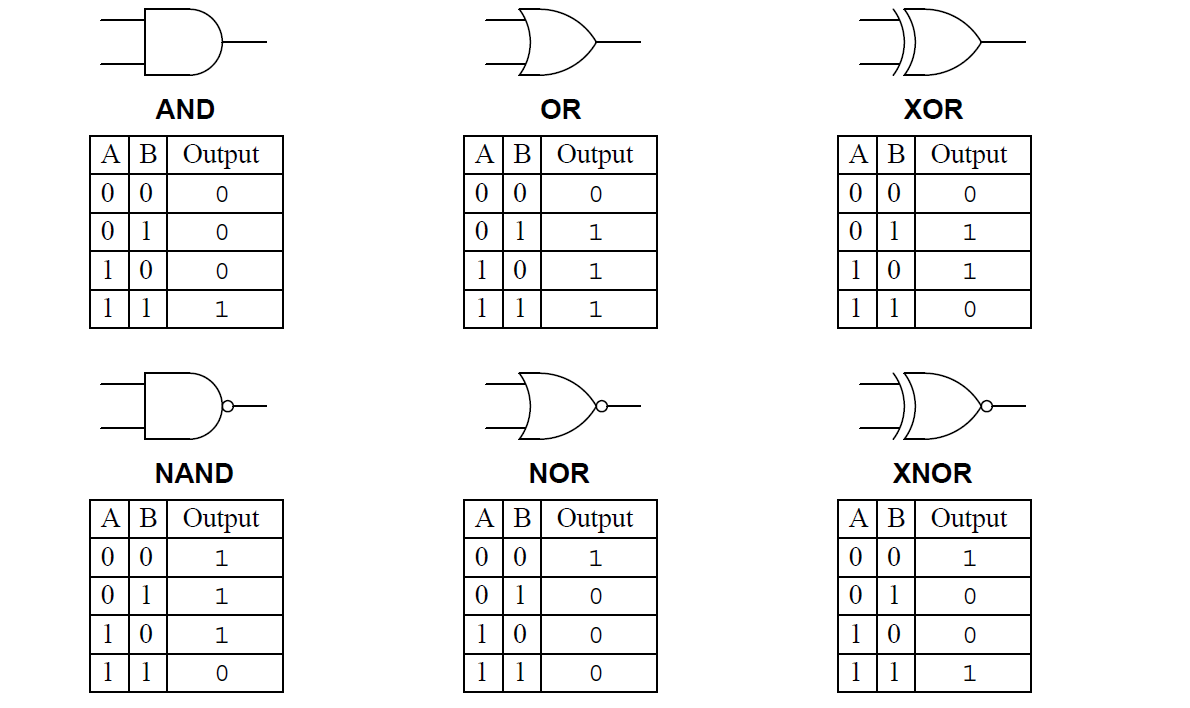
\includegraphics[width=\textwidth]{logic_gates.png}
\label{Logic Gates}
\end{figure}
\end{frame}

\begin{frame}
\frametitle{Adder}
\begin{figure}
\centering
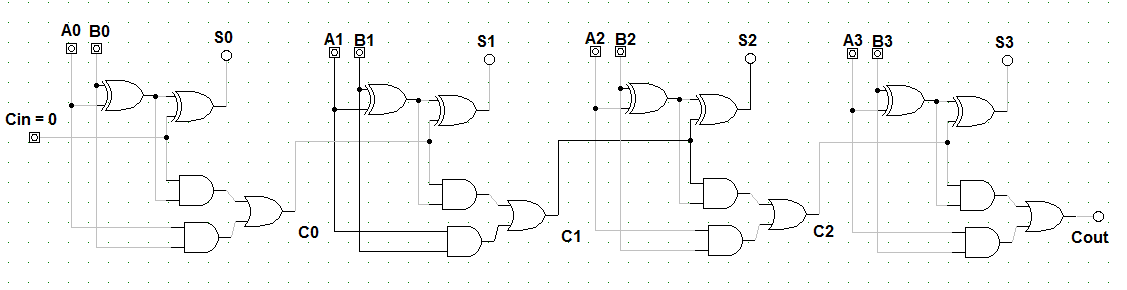
\includegraphics[width=\textwidth]{4bit_adder_3.png}
\label{Adder}
\end{figure}
\end{frame}

\end{document} 
